\documentclass[dvipdfmx]{jsarticle}
\usepackage[dvipdfmx]{hyperref, xcolor, graphicx}
\hypersetup{
    colorlinks=true,
    citecolor=blue,
    linkcolor=blue,
    urlcolor=blue,
}

% 数式
\usepackage{amsmath,amsfonts,amssymb,amsthm, mathtools}
\usepackage{bm}
\usepackage{physics}
\usepackage{tcolorbox}
\tcbuselibrary{breakable} % 必要に応じて

\newtcolorbox{mybox}[1][]{%
  title=#1,
  fonttitle=\gtfamily\sffamily\bfseries,
  colframe=blue,
  colback=blue!3!,
  breakable, % 長文対応したい場合
}

\usepackage[dvipdfmx]{graphicx}
\usepackage{tikz} %図を描く
\usetikzlibrary{positioning, intersections, calc, arrows.meta,math} 

\usepackage{here}

\begin{document}

\section{Bayes理論の目的}
Bayes理論は、パラメータの集合$W \subset \mathbb{R}^d$、真の分布$q(x)$、確率モデル$p(x|w)$、事前分布$\varphi(w)$が事前に与えられて構築される理論である。
理論の目的は以下のようにまとめられる:
\begin{mybox}[Bayes理論の目的]
    真の分布$q(x)$、確率モデル$p(x|w)$、事前分布$\varphi(w)$が与えられたとする。
    自然数$n=1,2,3,\ldots$に対して、我々は何らかの処方箋に従って予測分布と呼ばれる確率分布の系列$\{p_n^{*}(x)\}_{n=1}^{\infty}$を構成する。
    予測分布の構成手法はBayes推測、事後確率最大化法、最尤推定法、平均プラグイン法などが存在する。
    たとえばBayes推測を用いた場合では、予測分布を
    \begin{equation}
        p_{n}^{*}(x) \coloneqq \int p(x|w)p(w|X^n)\,\dd{w}
    \end{equation}
    と定める。
    ここで、$p(w|X^n)$は事後分布と呼ばれる確率分布であり、真の分布$q(x)$から得られる$n$個の独立なサンプル$X^n$(データセット)を用いて、
    \begin{equation}
        p(w|X^n) \propto \varphi(w)\prod_{i=1}^{n}p(X_i|w)^{\beta}
    \end{equation}
    と定義される。Bayes理論の主な目的は、予測分布の構成手法としてBayes推測を用いた場合、$n$の増大に対して
    \begin{equation}
        D_{\text{KL}}[q(x) \parallel p_n^{*}(x)] = \int q(x)\ln\frac{q(x)}{p_n^{*}(x)}\,\dd{x}
        \label{eq:bayes-goal}
    \end{equation}
    がどのような振る舞いをするか、すなわちどのように予測分布$p_n^*(x)$が真の分布$q(x)$に近づいていくかを調べることが目的である。
    また、複数のモデル・予測分布の構成手法に対して、それらの良し悪し(どのような意味での良し悪しかは後で)を定量的に評価できる情報量規準の導入も行う。
\end{mybox}
Bayes理論の目的にあるように、式\eqref{eq:bayes-goal}の$n$に対する振る舞いを調べていく。そのために必要な概念の定義を以下で行う。

\subsection{いくつかの概念の定義と本書の仮定について}

\begin{mybox}[真の分布に対して最適なパラメータの集合]
    パラメータの集合$W$に対し、真の分布$q(x)$とモデル$p(x|w)$の間のKL divergenceを最小にするパラメータの集合を$W_0$と定義する:
    \begin{equation}
        W_0 \coloneqq \{ w \in W \mid w = \arg\min_{w} D_{\mathrm{KL}}[q(x) \parallel p(x|w)] \}
    \end{equation}
    この集合のことを、真の分布に対して最適なパラメータの集合と呼ぶ。
\end{mybox}

\begin{mybox}[実質的にユニーク]
    任意の$w_0\in W_0$について、$p(x|w_0)$がユニークな確率分布$p_0(x)$を表すとき、真の分布に対して最適な確率分布は実質的にユニークであるという。
\end{mybox}
以下では実質的にユニークが常に実現されていることを仮定する。
さらにこの本では、より強い仮定として、「相対的に有限な分散を持つ」という状況が達成されていることを仮定する。
\footnote{「相対的に有限な分散を持つ」ことが達成されていない場合、後で定義する重要な量である$K_n(w)$の分散がその平均でバウンドできなくなるため、
事後分布がサンプルに応じて大きく変動してしまうことが問題となるらしいです。これ以上はよくわからないです。(渡辺ベイズ p36, 注意12を参照。)}

\begin{figure}[H]
    \centering
    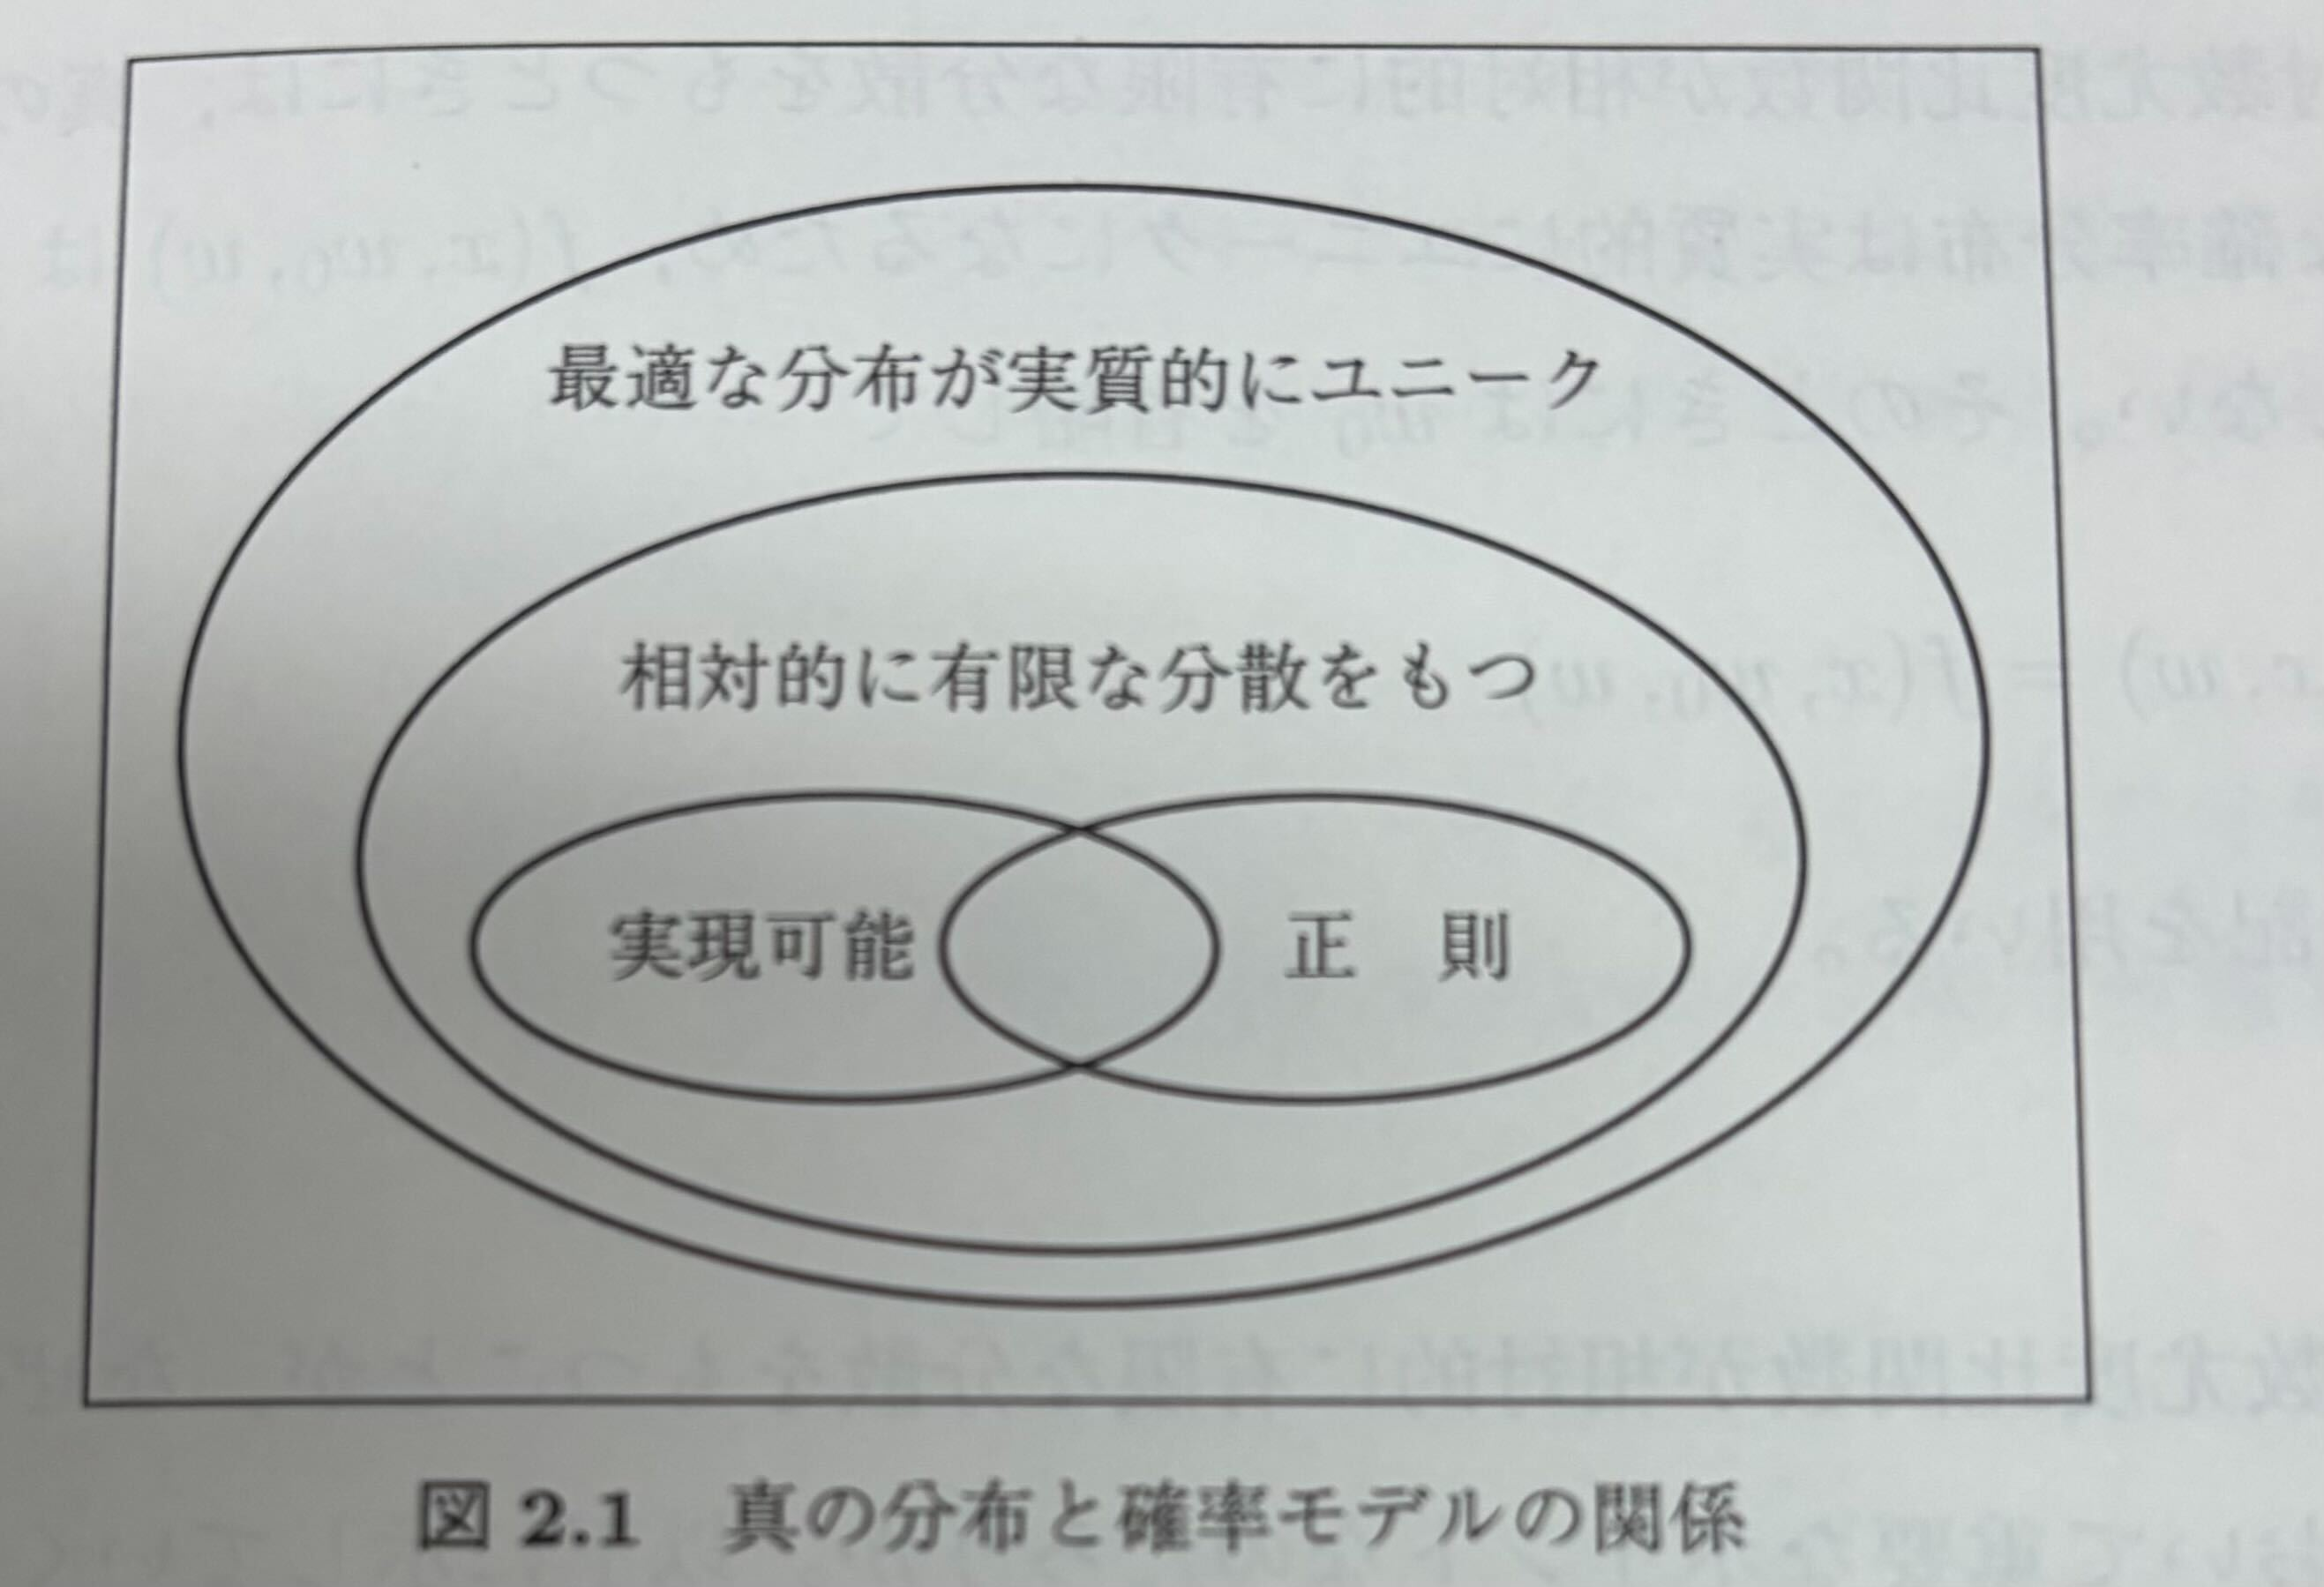
\includegraphics[width=0.5\textwidth]{yuugennnabunsan.jpg}
    \caption{真の分布と確率モデルに対する関係(渡辺ベイズ p35)}
    \label{fig:katei}
\end{figure}
以下の説明は、「相対的に有限な分散を持つ」ことが達成されている、すなわち「最適な分布が実質的にユニーク」な状況を前提にしている。
したがって、真の分布$q(x)$にKL divergenceの意味で最も近い確率モデルは唯一$p_0(x)$に定まっている。

\subsection{Bayes理論の目的を達成するために必要なこと}
Bayes理論の目的は、$D_{\text{KL}}[q(x) \parallel p_n^{*}(x)]$の$n$に対する振る舞いを調べることである。
以下では計算の都合上、式\eqref{eq:bayes-goal}の両辺から$D_{\text{KL}}[q(x) \parallel p_0(x)]$($n$にはよらない定数)を引いた値の振る舞いを考える:

\begin{equation}
    D_{\text{KL}}[q(x) \parallel p_n^{*}(x)] - D_{\text{KL}}[q(x) \parallel p_0(x)] = -\int q(x) \ln\frac{p_n^{*}(x)}{p_0(x)}\dd{x}\;。
\end{equation}
予測分布の構成方法としてBayes推測を用いた場合、右辺は
\begin{equation}
    -\int q(x) \ln\frac{p_n^{*}(x)}{p_0(x)}\,\dd{x} = -\mathbb{E}_{X}\qty[\ln \ev{e^{\ln\frac{p(X|w)}{p(X|w_0)}}}_{w|X^n}]
    \label{eq:bayes-sekibun}
\end{equation}
と表される。なお、$\ev{\cdots}_{w|X^n}$は事後分布による期待値を表す:
\begin{equation}
    \ev{O(x,w)}_{w|X^n} \coloneqq \int O(x,w)p(w|X^n)\,\dd{w}\;。
    \label{eq:expectation}
\end{equation}
式\eqref{eq:bayes-sekibun}の$n$の増大に対する振る舞いを見るためには、式\eqref{eq:expectation}の$n$に対する振る舞いを調べることがすべてである。
その調査を行えるようにするため、$p(w|X^n)$を天下り的だが($w$の積分計算にラプラス近似を用いたいため)次のように変形する:
\begin{equation}
    p(w|X^n)\propto \varphi(w)\prod_{i=1}^{n}p(X_i|w)^{\beta} \propto \varphi(w)\exp(-n\beta K_n(w))\;。
\end{equation}
ここで$K_n(w)$は経験誤差関数であり、
\begin{equation}
    K_n(w) \coloneqq \frac{1}{n}\sum_{i=1}^{n}f(X_i,w) \coloneqq \frac{1}{n}\sum_{i=1}^{n} \ln{\frac{p(X_i|w_0)}{p(X_i|w)}}
\end{equation}
と定義される。なお、$f(x,w)$は対数尤度比関数と呼ばれる。
このように変形することで、事後分布の確率的な振る舞いを$K_n(w)$に押し付けることができた。さらに指数関数の肩が$-n$に比例しているため、
$n$が十分に大きな場合、式\eqref{eq:expectation}の積分計算に寄与する領域は$K_n(w)$の最小値付近のみと考えることができる。したがって、
\begin{enumerate}
    \item $K_n(w)$の最小値を取る点が、パラメータ空間$W$全体でどのような分布をしているか
    \item $K_n(w)$の最小値周りにおける関数の局所的な振る舞い
\end{enumerate}
を調べることが重要である。
$K_n(w)$の$w$に対する振る舞い方は、真の分布とモデル設計に依存して決まるため、まずは正則理論という枠組みの元で$K_n(w)$の振る舞いを考える。

\section{正則理論}
正則理論とは、以下の3つの条件を真の分布とモデル設計に課す理論である:
\begin{enumerate}
    \item 最適なパラメータの集合は唯一の元からなる:
    \begin{equation}
        W_0 = \{w_0\}\;。
    \end{equation}
    これは$K(w)$を最小にするパラメータが唯一$w_0$であることと同値である。
    \item $K(w)$のヘシアン$\laplacian{K(w)}$の$w=w_0$における値が正定値である。
    \item サンプルの数$n$が非常に大きいこと。
\end{enumerate}

正則理論の

\section{正則理論の場合}





天下り的ではあるが、$K_n(w)$を次のように変形する:
\begin{equation}
    K_n(w) = K(w) - (K(w)-K_n(w)) = K(w) - \frac{1}{\sqrt{n}}\eta_n(w)\;。
\end{equation}
ここで






\begin{mybox}[事後分布の振る舞い(正則理論の場合)]
    正則理論という仮定を課している場合、式\eqref{eq:expectation}の振る舞いは次のように表される:
    \begin{equation}
        \ev{O(x,w)}_{w|X^n}
         = \frac{\int O(x,w)\exp(-\frac{n\beta}{2}\abs{J^{1/2}(w-w_0-\frac{\hat{\xi_n}}{\sqrt{n}})})dw}
         {\int \exp(-\frac{n\beta}{2}\abs{J^{1/2}(w-w_0-\frac{\hat{\xi_n}}{\sqrt{n}})})dw}(1+o_p(1))
    \end{equation}
\end{mybox}


\end{document}
